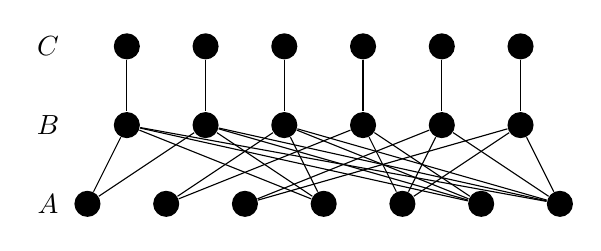
\begin{tikzpicture}
\foreach \x/\t in {2/A,1/B,0/C} {
  \node (T\x) at (0,-\x) {$\t$};
}
\foreach \x in {1,...,6} {
  \node[fill,circle] (C\x) at (\x,0) {};
  \node[fill,circle] (B\x) at (\x,-1) {};
  \draw (C\x) -- (B\x);
}
\foreach \x in {0,...,6} {
  \node[fill,circle] (A\x) at (\x+0.5,-2) {};
}
\foreach \xa/\xb in {0/1,0/2,1/3,1/4,2/5,2/6,3/1,3/2,3/3,4/4,4/5,4/6,5/1,5/2,5/3,5/4,6/5,6/6,6/1,6/2,6/3} {
  \draw (A\xa) -- (B\xb);
}
\end{tikzpicture}